% !TEX TS-program = xelatex
\documentclass[aspectratio=169, 10pt, table]{beamer}
\usefonttheme{professionalfonts}

\usepackage{fontspec}
\usepackage{polyglossia}
\setmainlanguage{french}
\usepackage{graphicx}
\usepackage{booktabs}
\usepackage{tabularx}
\usepackage{colortbl}
\usepackage{tikz}
\usepackage[export]{adjustbox}
\usepackage{hyperref}
\urlstyle{same}
\usepackage{microtype}
\usetikzlibrary{shapes.geometric, shapes.misc, arrows.meta, positioning, calc, shadows}

% Fonts
\IfFontExistsTF{Liberation Sans Narrow}{
    \setmainfont{Liberation Sans Narrow}
    \setsansfont{Liberation Sans Narrow}
}{
    \IfFontExistsTF{Arial Narrow}{
        \setmainfont{Arial Narrow}
        \setsansfont{Arial Narrow}
    }{
        \setsansfont{TeX Gyre Heros}
    }
}
\IfFontExistsTF{Liberation Mono}{
    \setmonofont{Liberation Mono}
}{
    \IfFontExistsTF{DejaVu Sans Mono}{
        \setmonofont{DejaVu Sans Mono}
    }{}
}

% Official Colors Télécom SudParis
\definecolor{TSPblue}{HTML}{0052A0}
\definecolor{TSPcyan}{HTML}{00A3E0}
\definecolor{TSPblack}{HTML}{1D1D1B}
\definecolor{TSPdark}{RGB}{128, 0, 32}
\definecolor{TSPgrey}{HTML}{F0F0F0}
\definecolor{TSPtext}{HTML}{333333}

% Theme configuration
\setbeamercolor{normal text}{fg=TSPtext,bg=white}
\setbeamercolor{title}{fg=TSPblue}
\setbeamercolor{subtitle}{fg=TSPcyan}
\setbeamercolor{author}{fg=TSPblue}
\setbeamercolor{institute}{fg=TSPblue}
\setbeamercolor{date}{fg=TSPblue}
\setbeamercolor{frametitle}{fg=TSPblue}
\setbeamercolor{section in head/foot}{fg=TSPblue}
\setbeamercolor{footline}{bg=TSPgrey,fg=TSPtext}
\setbeamercolor{section in toc}{fg=TSPblue!35}
\setbeamercolor{section in toc shaded}{fg=TSPblue!35}

\setbeamertemplate{navigation symbols}{}

\setbeamertemplate{section in toc}{%
  \ifnum\inserttocsectionnumber=\insertsectionnumber
    \textcolor{TSPblue}{\textbf{\inserttocsectionnumber. \inserttocsection}}
  \else
    \textcolor{TSPblue!35}{\inserttocsectionnumber. \inserttocsection}
  \fi
}

\setbeamertemplate{frametitle}{%
    \vspace*{0.25cm}%
    {\usebeamerfont{frametitle}\usebeamercolor[fg]{frametitle}\textbf{\insertframetitle}}\par%
    \vspace*{0.15cm}%
    {\color{TSPdark}\hrule height 0.8pt}%
}

% Header template
\setbeamertemplate{headline}{%
    \ifnum\thepage>1
    \vspace{0.15cm}
    \hspace{0.03\textwidth}
    \begin{minipage}[c]{0.12\textwidth}
        \IfFileExists{tsp_logo.png}{
            
\includegraphics[height=0.6cm,keepaspectratio]{tsp_logo.png}
        }{
            \fbox{\tiny TSP}
        }
    \end{minipage}
    \hfill
    \begin{minipage}[c]{0.80\textwidth}
        \raggedleft
        \usebeamerfont{section in head/foot}\color{TSPblue}
        \scriptsize\insertsectionhead
    \end{minipage}
    \hspace{0.03\textwidth}
    \vspace{0.1cm}
    \fi
}

% Footline template
\setbeamertemplate{footline}{%
    \ifnum\thepage>1
    \begin{beamercolorbox}[wd=\paperwidth,ht=2.2ex,dp=1ex,leftskip=0.03\textwidth,rightskip=0.03\textwidth]{footline}%
        \tiny
        \textbf{Télécom SudParis} \hfill
        Sécurité de l'IA Générative --- Sprint 2 \hfill
        \insertframenumber
    \end{beamercolorbox}%
    \fi
}

% Blocks styling
\setbeamercolor{block title}{bg=TSPblue,fg=white}
\setbeamercolor{block body}{bg=TSPgrey,fg=TSPtext}
\setbeamercolor{block title alerted}{bg=TSPdark,fg=white}
\setbeamercolor{block body alerted}{bg=TSPgrey,fg=TSPtext}

\setbeamertemplate{block begin}{
  \vskip\smallskipamount
  \begin{beamercolorbox}[leftskip=1ex,colsep*=.75ex]{block title}
    \usebeamerfont*{block title}\textbf{\insertblocktitle}
  \end{beamercolorbox}%
  {\ifbeamercolorempty[bg]{block body}{}{\nointerlineskip\vskip-0.5pt}}%
  \usebeamerfont{block body}%
  \begin{beamercolorbox}[dp=1ex,leftskip=1ex,vmode,colsep*=.75ex]{block body}%
    \ifbeamercolorempty[bg]{block body}{\vskip-.25ex}{\vskip-.75ex}\vbox{}%
    \raggedright\hyphenpenalty=10000
}
\setbeamertemplate{block end}{
  \end{beamercolorbox}\vskip\smallskipamount
}

\setbeamertemplate{block alerted begin}{
  \vskip\smallskipamount
  \begin{beamercolorbox}[leftskip=1ex,colsep*=.75ex]{block title alerted}
    \usebeamerfont*{block title alerted}\textbf{\insertblocktitle}
  \end{beamercolorbox}%
  {\ifbeamercolorempty[bg]{block body alerted}{}{\nointerlineskip\vskip-0.5pt}}%
  \usebeamerfont{block body}%
  \begin{beamercolorbox}[dp=1ex,leftskip=1ex,vmode,colsep*=.75ex]{block body alerted}%
    \ifbeamercolorempty[bg]{block body alerted}{\vskip-.25ex}{\vskip-.75ex}\vbox{}%
    \raggedright\hyphenpenalty=10000
}
\setbeamertemplate{block alerted end}{
  \end{beamercolorbox}\vskip\smallskipamount
}

% Environment hyphenation fixes
\AtBeginEnvironment{frame}{\raggedright\hyphenpenalty=10000}
\AtBeginEnvironment{itemize}{\raggedright\hyphenpenalty=10000}
\AtBeginEnvironment{tabularx}{\raggedright\hyphenpenalty=10000}
\AtBeginEnvironment{column}{\raggedright\hyphenpenalty=10000}

% Macros
\newcommand{\cnum}[1]{\tikz[baseline=-0.8ex]\node[circle, fill=TSPblue, text=white, inner sep=1pt, font=\scriptsize\bfseries]{#1};}
\newcommand{\cnumdark}[1]{\tikz[baseline=-0.8ex]\node[circle, fill=TSPdark, text=white, inner sep=1pt, font=\scriptsize\bfseries]{#1};}

% Title page (exactement identique a presentation_latex/main.tex)
\setbeamertemplate{title page}{
    \centering
    \vspace*{2ex}
    \IfFileExists{tsp_logo.png}{
        
\includegraphics[height=1.5cm]{tsp_logo.png}
    }{
        \fbox{tsp\_logo.png}
    }
    \vfill

    {\usebeamercolor[fg]{title}\huge\textbf{Sécurité de l'IA Générative}\par}
    \vspace*{1ex}
    {\usebeamercolor[fg]{subtitle}\large Étude de la mémorisation dans les modèles génératifs\par}
    \vspace*{1ex}
    {\fontsize{9}{11}\selectfont Liens avec le surapprentissage et implications pour la confidentialité des données, un angle sécurité\par}
    \vfill
    {\fontsize{10}{12}\selectfont
    \textbf{Présenté par :} Emmanuel SININI et Fatima-Zahra Rhoulam\par
    \vspace*{0.8ex}
    \textbf{Encadrants :} Maryline Laurent (TSP) $\cdot$ Faiz Taleb (TSP / EDF)\par}
    \vspace*{1ex}
    {\fontsize{11}{13}\selectfont \textbf{Télécom SudParis}\par}
    \vspace*{1ex}
    {\fontsize{10}{12}\selectfont 1\textsuperscript{ère} réunion de projet\par}
    \vfill
}

\AtBeginSection[]{
  \begin{frame}{Plan}
    \tableofcontents
  \end{frame}
}

\begin{document}

% -----------------------------------------------------------------------------
% SLIDE DE TITRE
% -----------------------------------------------------------------------------
\begin{frame}[plain]
    \titlepage
\end{frame}

% -----------------------------------------------------------------------------
% SECTION 1 : CLASSIFICATION D'IMAGES (CNN CIFAR-10) — PERIMETRE FATIMA-ZAHRA
% -----------------------------------------------------------------------------
\section{Classification d'Images (CNN CIFAR-10)}

\begin{frame}{CNN --- Architecture \& Forward Pass}
    \centering
    \vspace{-0.25cm}
    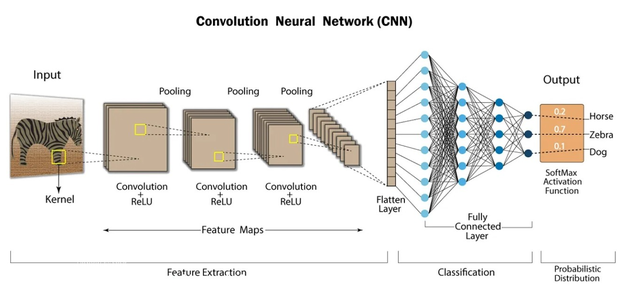
\includegraphics[max width=0.82\textwidth, max height=0.33\textheight, keepaspectratio]{cnn_architecture.png}\par
    \vspace{0.04cm}
    {\scriptsize \textbf{Architecture générale d'un CNN :} extraction de caractéristiques \& classification}\par
    \vspace{0.02cm}
    {\tiny\color{TSPtext!70}Source : N. Shahriar, \textit{"What is Convolutional Neural Network (CNN) in Deep Learning?"} $\cdot$ LinkedIn}\par
    \vspace{0.12cm}
    \small
    \begin{itemize}
        \setlength{\itemsep}{1pt}
        \item \textbf{\color{TSPblue}Convolution :} Filtres détectant les motifs locaux hiérarchiques (contours, textures).
        \item \textbf{\color{TSPblue}Pooling :} Réduction spatiale assurant la robustesse aux translations.
        \item \textbf{\color{TSPblue}Softmax :} $\text{Softmax}(z_i) = \frac{\exp(z_i)}{\sum_j \exp(z_j)} \implies$ distribution prédictive sur les classes.
    \end{itemize}
\end{frame}

\begin{frame}{CNN --- La Fonction de Perte comme Origine du Signal}
    \begin{columns}[T]
        \begin{column}{0.50\textwidth}
            \begin{block}{Cross-Entropy Loss (Entropie Croisée)}
                \small
                $$\mathcal{L}_{\text{CE}} = - \log\big(p_{\text{classe correcte}}\big)$$
                \vspace{-0.2cm}
                \begin{itemize}
                    \item Minimisation stricte sur les exemples d'entraînement.
                    \item \textbf{Image Train :} $p_{\max} \to 1 \implies \mathcal{L}_{\text{CE}} \approx 0$.
                    \item \textbf{Image Test (inédite) :} $p_{\max}$ modéré $\implies \mathcal{L}_{\text{CE}}$ nettement plus élevée.
                \end{itemize}
            \end{block}
        \end{column}

        \begin{column}{0.46\textwidth}
            \begin{alertblock}{Conséquence Opérationnelle (Surapprentissage)}
                \small
                L'\textbf{écart de confiance} entre train et test constitue la définition opérationnelle du surapprentissage.
                \begin{itemize}
                    \item Le réseau est « sur-confiant » sur les données vues.
                    \item Cet écart résiduel est le \textbf{signal fondamental} exploité par les attaques d'inférence (MIA).
                \end{itemize}
            \end{alertblock}
            \vspace{0.15cm}
            {\scriptsize Réf : Shokri et al. (IEEE S\&P 2017) $\cdot$ Yeom et al. (IEEE CSF 2018)}
        \end{column}
    \end{columns}
\end{frame}

\begin{frame}{CNN --- Attaque Déduite : Membership Inference (MIA)}
    \centering
    \vspace{-0.1cm}
    \begin{tikzpicture}[
        scale=0.88, transform shape,
        box/.style={rectangle, draw=TSPblue, rounded corners, fill=white, text width=2.4cm, align=center, minimum height=0.75cm, font=\scriptsize, shadow xshift=1pt, shadow yshift=-1pt, drop shadow={opacity=0.2}},
        darkbox/.style={box, fill=TSPblue, text=white, draw=TSPblue},
        alertbox/.style={box, fill=TSPdark, text=white, draw=TSPdark},
        arr/.style={-{Stealth[scale=0.85]}, thick, TSPblue}
    ]
        \node[box] (n1) {\textbf{1. Donnée cible} $x$\\[1pt]\tiny IN ou OUT ?};
        \node[box, right=0.35cm of n1] (n2) {\textbf{2. Requête CNN}\\[1pt]\tiny Vecteur $p$ ou $\mathcal{L}$};
        \node[darkbox, right=0.35cm of n2] (n3) {\textbf{3. Signal}\\[1pt]\tiny $p_{\max}$ ou $-\log p$};
        \node[darkbox, right=0.35cm of n3] (n4) {\textbf{4. Seuil calibré}\\[1pt]\tiny $\tau$ (Shadow / Yeom)};
        \node[alertbox, right=0.35cm of n4] (n5) {\textbf{5. Verdict}\\[1pt]\tiny IN si signal $\le \tau$};

        \draw[arr] (n1) -- (n2);
        \draw[arr] (n2) -- (n3);
        \draw[arr] (n3) -- (n4);
        \draw[arr] (n4) -- (n5);
    \end{tikzpicture}

    \vspace{0.25cm}
    \begin{itemize}
        \item \textbf{\color{TSPblue}Shokri et al. (IEEE S\&P 2017) :} Entraînement de multiples \emph{shadow models} mimant le comportement du modèle cible, puis apprentissage d'un classifieur d'attaque supervisé.
        \item \textbf{\color{TSPblue}Yeom et al. (IEEE CSF 2018) :} Seuil analytique direct sur la perte : $\mathcal{M}(x) = \mathbb{I}(\mathcal{L}(x) \le \tau)$.
        \item \textbf{\color{TSPdark}Lien théorique :} L'avantage de l'attaquant est directement borné par l'écart de généralisation : $\text{Adv} \le \text{Acc}_{\text{train}} - \text{Acc}_{\text{test}}$.
    \end{itemize}
\end{frame}

\begin{frame}{Shadow Models \& Classifieur d'Attaque (Shokri et al.)}
    \centering
    \vspace{-0.1cm}
    \begin{figure}[htbp]
        \centering
        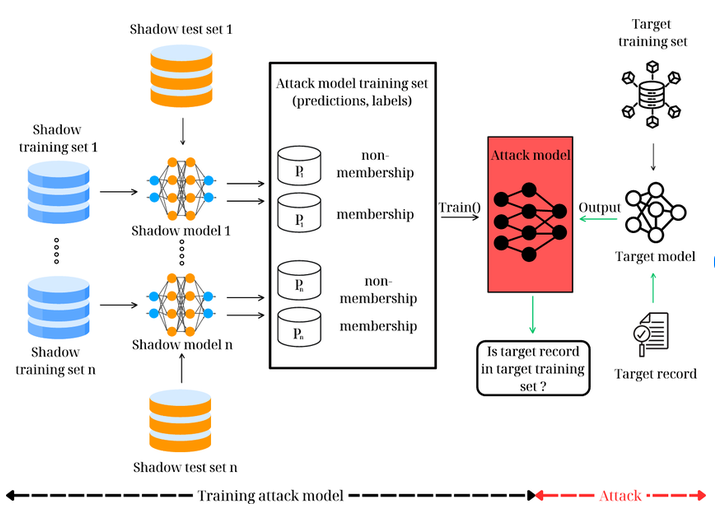
\includegraphics[max width=0.88\textwidth, max height=0.62\textheight, keepaspectratio]{shadow-models.png}
        \caption{\footnotesize Workflow des attaques par inférence d'appartenance (MIA) via \emph{Shadow Models}.}
        \vspace{0.1cm}
        {\tiny\color{TSPtext!70} 
            Source : C. C. Nikolaidis, \textit{"A study of membership inference attacks on a federated health care application"}, 
            Computing 107(7), 2025. \href{https://doi.org/10.1007/s00607-025-01507-x}{\texttt{DOI: 10.1007/s00607-025-01507-x}}
        }
    \end{figure}
\end{frame}


\begin{frame}{CNN --- Analyse Empirique : Exemple Chiffré sur CIFAR-10}
    \begin{columns}[c]
        \begin{column}{0.52\textwidth}
            \renewcommand{\arraystretch}{1.25}
            \small
            \begin{tabularx}{\textwidth}{>{\bfseries}l >{\centering\arraybackslash}X >{\centering\arraybackslash}X}
                \toprule
                \rowcolor{TSPblue}\color{white}\textbf{Métrique observée} & \color{white}\textbf{Image Train (IN)} & \color{white}\textbf{Image Test (OUT)} \\
                \midrule
                Confiance $p_{\max}$ (« chat ») & \textbf{0{,}994} & 0{,}710 \\
                Perte $\mathcal{L}_{\text{CE}} = -\log(p_{\max})$ & \textbf{0{,}006} & 0{,}342 \\
                Ratio de perte (Test / Train) & \multicolumn{2}{c}{\textbf{Facteur 57$\times$ d'écart}} \\
                \midrule
                Verdict ($\tau = 0{,}05$) & \textbf{\color{TSPblue}IN (Correct)} & \textbf{\color{TSPdark}OUT (Correct)} \\
                \bottomrule
            \end{tabularx}
        \end{column}

        \begin{column}{0.45\textwidth}
            \begin{alertblock}{Constat d'Exploitation}
                \small
                \begin{itemize}
                    \item Avec un seuil calibré $\tau = 0{,}05$, l'attaquant sépare parfaitement les deux images.
                    \item \textbf{Origine physique :} L'optimisation force la convergence des poids vers les détails stochastiques d'entraînement (bruit haute fréquence propre au train set).
                \end{itemize}
            \end{alertblock}
        \end{column}
    \end{columns}
\end{frame}

% -----------------------------------------------------------------------------
% SECTION 2 : SERIES TEMPORELLES (LSTM) — PERIMETRE FATIMA-ZAHRA
% -----------------------------------------------------------------------------
\section{Séries Temporelles (LSTM)}

\begin{frame}{LSTM --- Architecture \& Forward Pass}
    \centering
    \vspace{-0.1cm}
    \begin{tikzpicture}[
        scale=0.90, transform shape,
        box/.style={rectangle, draw=TSPblue, rounded corners, fill=white, text width=2.5cm, align=center, minimum height=0.75cm, font=\scriptsize, shadow xshift=1pt, shadow yshift=-1pt, drop shadow={opacity=0.2}},
        darkbox/.style={box, fill=TSPblue, text=white, draw=TSPblue},
        arr/.style={-{Stealth[scale=0.85]}, thick, TSPblue}
    ]
        \node[box] (f) {\textbf{Porte d'oubli}\\$f_t = \sigma(W_f x_t + U_f h_{t-1})$};
        \node[box, right=0.35cm of f] (i) {\textbf{Porte d'entrée}\\$i_t = \sigma(W_i x_t + U_i h_{t-1})$};
        \node[darkbox, right=0.35cm of i] (c) {\textbf{Mémoire cellulaire}\\$C_t = f_t \odot C_{t-1} + i_t \odot \tilde{C}_t$};
        \node[box, right=0.35cm of c] (o) {\textbf{Porte de sortie}\\$o_t = \sigma(W_o x_t + U_o h_{t-1})$};
        \node[darkbox, right=0.35cm of o] (pred) {\textbf{Prédiction}\\$\hat{x}_{t+1} = W_y h_t$};

        \draw[arr] (f) -- (i);
        \draw[arr] (i) -- (c);
        \draw[arr] (c) -- (o);
        \draw[arr] (o) -- (pred);
    \end{tikzpicture}

    \vspace{0.25cm}
    $$C_t = f_t \odot C_{t-1} + i_t \odot \tilde{C}_t$$
    \vspace{-0.1cm}
    \begin{itemize}
        \item \textbf{\color{TSPblue}Porte d'oubli $f_t$ :} Proportion d'information conservée de l'état passé $C_{t-1}$.
        \item \textbf{\color{TSPblue}Porte d'entrée $i_t$ :} Degré de mise à jour par la nouvelle entrée $\tilde{C}_t$.
        \item \textbf{\color{TSPblue}Porte de sortie $o_t$ :} Exposition sélective de la mémoire cellulaire vers $h_t \to \hat{x}_{t+1}$.
    \end{itemize}
\end{frame}

\begin{frame}{LSTM --- L'Erreur de Prédiction MSE comme Signal}
    \begin{columns}[T]
        \begin{column}{0.48\textwidth}
            \begin{block}{Erreur Quadratique Moyenne (\texttt{MSE})}
                \small
                $$\mathcal{L}_{\text{MSE}} = \big(\hat{x}_{t+1} - x_{t+1}\big)^2$$
                \vspace{-0.2cm}
                \begin{itemize}
                    \item Optimisation par rétropropagation à travers le temps (BPTT).
                    \item \textbf{Séquence Train :} Erreur résiduelle anormalement basse ($< 10^{-3}$).
                    \item \textbf{Séquence Test :} Erreur de prédiction nettement plus élevée en moyenne.
                \end{itemize}
            \end{block}
        \end{column}

        \begin{column}{0.48\textwidth}
            \begin{block}{Analogie avec la Perplexité des LLM}
                \small
                Pour une série temporelle continue, l'erreur MSE joue le rôle exact de la \textbf{perplexité} :
                \begin{itemize}
                    \item Elle quantifie la \textbf{surprise} locale du réseau face à la dynamique observée.
                    \item Un résidu proche de zéro trahit une mémorisation mécanique de la série temporelle.
                \end{itemize}
            \end{block}
        \end{column}
    \end{columns}
\end{frame}

\begin{frame}{LSTM --- Attaque Déduite : Canaris \& Métrique d'Exposure}
    \centering
    \vspace{-0.1cm}
    \begin{tikzpicture}[
        scale=0.88, transform shape,
        box/.style={rectangle, draw=TSPblue, rounded corners, fill=white, text width=2.4cm, align=center, minimum height=0.75cm, font=\scriptsize, shadow xshift=1pt, shadow yshift=-1pt, drop shadow={opacity=0.2}},
        darkbox/.style={box, fill=TSPblue, text=white, draw=TSPblue},
        alertbox/.style={box, fill=TSPdark, text=white, draw=TSPdark},
        arr/.style={-{Stealth[scale=0.85]}, thick, TSPblue}
    ]
        \node[box] (n1) {\textbf{1. Injection}\\[1pt]\tiny Canari rare ($N$ copies)};
        \node[box, right=0.35cm of n1] (n2) {\textbf{2. Entraînement}\\[1pt]\tiny Checkpoints 20/100/200};
        \node[darkbox, right=0.35cm of n2] (n3) {\textbf{3. Requête}\\[1pt]\tiny MSE sur canari réel};
        \node[darkbox, right=0.35cm of n3] (n4) {\textbf{4. Comparaison}\\[1pt]\tiny Contre $K$ variantes};
        \node[alertbox, right=0.35cm of n4] (n5) {\textbf{5. Exposure}\\[1pt]\tiny Rang dans la distribution};

        \draw[arr] (n1) -- (n2);
        \draw[arr] (n2) -- (n3);
        \draw[arr] (n3) -- (n4);
        \draw[arr] (n4) -- (n5);
    \end{tikzpicture}

    \vspace{0.25cm}
    \begin{itemize}
        \item \textbf{\color{TSPblue}Protocole \emph{The Secret Sharer} (Carlini et al., USENIX 2019) :} Insertion d'un motif temporel rare et génération de variantes fictives candidates.
        \item \textbf{\color{TSPblue}Formule de l'Exposure :} $\text{Exposure}(s) = \log_2 |Q| - \log_2 \text{Rang}(s)$.
        \item \textbf{\color{TSPdark}Interprétation :} Un rang de 1 signifie que le canari est dissociable de tout le bruit de fond, prouvant une mémorisation absolue dans les poids du modèle.
    \end{itemize}
\end{frame}

\begin{frame}{LSTM --- Exemple Chiffré \& Évolution par Époque}
    \begin{columns}[c]
        \begin{column}{0.52\textwidth}
            \renewcommand{\arraystretch}{1.25}
            \small
            \begin{tabularx}{\textwidth}{>{\bfseries}l >{\centering\arraybackslash}X}
                \toprule
                \rowcolor{TSPblue}\color{white}\textbf{Mesure Expérimentale} & \color{white}\textbf{Valeur Observée} \\
                \midrule
                MSE sur le canari secret exact & \textbf{0{,}0004} \\
                MSE moyenne sur les séquences de test & \textbf{0{,}1830} \\
                Ratio de résidu (Test / Canari) & \textbf{Facteur 450$\times$} \\
                \midrule
                Rang du canari parmi 10 variantes & \textbf{\color{TSPblue}1$^{\text{er}}$ / 10} \\
                \bottomrule
            \end{tabularx}
        \end{column}

        \begin{column}{0.45\textwidth}
            \begin{alertblock}{Dynamique Temporelle d'Apparition}
                \small
                \begin{itemize}
                    \item \textbf{À 20 époques :} Le canari est confondu avec le bruit ($\text{Rang} \approx 6/10$).
                    \item \textbf{À 100 époques :} Décrochage net de la MSE ($\text{Rang} \to 2/10$).
                    \item \textbf{À 200 époques :} Mémorisation stricte ($\text{Rang} = 1/10$).
                \end{itemize}
                On capture précisément le point de bascule où le surapprentissage s'installe.
            \end{alertblock}
        \end{column}
    \end{columns}
\end{frame}

% -----------------------------------------------------------------------------
% SECTION 3 : GENERATION TEXTUELLE (NANOGPT) — PERIMETRE EMMANUEL
% -----------------------------------------------------------------------------
\section{Génération Textuelle (NanoGPT)}

\begin{frame}{Anatomie de NanoGPT : La Factorisation Autorégressive}
    \begin{columns}[T]
        \begin{column}{0.52\textwidth}
            \textbf{Principe du Transformer Causal :}
            \vspace{-0.1cm}
            $$P(X) = \prod_{t=1}^N P(x_t \mid x_{<t})$$
            \vspace{-0.3cm}
            \small
            \begin{itemize}
                \item \textbf{Entrée :} Contexte passé $x_{1:t}$.
                \item \textbf{Attention causale :} Masque triangulaire strict empêchant la vision future.
                \item \textbf{Logits \& Softmax :} $P(x_{t+1} = w) = \frac{\exp(z_w / T)}{\sum_j \exp(z_j / T)}$.
                \item \textbf{Génération récursive :} Concaténation séquentielle de $x_{t+1}$.
            \end{itemize}
        \end{column}

        \begin{column}{0.45\textwidth}
            \begin{block}{Code source clé : \texttt{model.py} (L.283)}
                \scriptsize
                \texttt{for \_ in range(max\_new\_tokens):}\\
                \quad\texttt{logits, \_ = self(idx\_cond)}\\
                \quad\texttt{logits = logits[:, -1, :] / temperature}\\
                \quad\texttt{probs = F.softmax(logits, dim=-1)}\\
                \quad\texttt{idx\_next = torch.multinomial(probs, 1)}\\
                \quad\texttt{idx = torch.cat((idx, idx\_next), dim=1)}
            \end{block}
            \vspace{0.15cm}
            {\scriptsize Dépôt officiel : \url{https://github.com/karpathy/nanoGPT}}
        \end{column}
    \end{columns}
\end{frame}

\begin{frame}{Pipeline de Décision Autorégressif (NanoGPT)}
    \centering
    \vspace{-0.15cm}
    \begin{tikzpicture}[
        node distance=0.25cm and 0.35cm,
        box/.style={rectangle, draw=TSPblue, rounded corners, fill=white, text width=4.3cm, align=center, minimum height=0.75cm, shadow xshift=1pt, shadow yshift=-1pt, drop shadow={opacity=0.25}, font=\scriptsize},
        darkbox/.style={box, fill=TSPblue, text=white, draw=TSPblue},
        alertbox/.style={box, fill=TSPdark, text=white, draw=TSPdark},
        arrow/.style={-{Stealth[scale=1.0]}, thick, TSPblue}
    ]
        \node[box] (1) {\cnum{1} \textbf{Prompt / Contexte initial} \\ Séquence de tokens $x_{1:t}$};
        \node[box, below=of 1] (2) {\cnum{2} \textbf{Attention Causale + MLP} \\ Pondération contextuelle};
        \node[box, below=of 2] (3) {\cnum{3} \textbf{Tête Linéaire \& Logits} \\ Logits $z \in \mathbb{R}^{|V|}$};

        \node[darkbox, right=of 1] (4) {\cnum{4} \textbf{Softmax \& Température $T$} \\ Distribution $P(x_{t+1})$};
        \node[darkbox, below=of 4] (5) {\cnum{5} \textbf{Échantillonnage multinomial} \\ Nouveau token $x_{t+1}$};
        \node[alertbox, below=of 5] (6) {\cnumdark{6} \textbf{Boucle Autorégressive} \\ \texttt{idx = torch.cat([idx, idx\_next])}};

        \draw[arrow] (1) -- (2);
        \draw[arrow] (2) -- (3);
        \draw[arrow] (3.east) to[out=0, in=180] (4.west);
        \draw[arrow] (4) -- (5);
        \draw[arrow] (5) -- (6);
        \draw[-{Stealth[scale=1.0]}, thick, dashed, TSPdark] (6.west) to[out=180, in=0] (1.south east);
    \end{tikzpicture}

    \vspace{0.15cm}
    {\footnotesize\color{TSPdark}\textbf{Faille structurelle :} Dès qu'un token mémorisé domine ($z_w \gg z_j$), la boucle s'auto-renforce de manière déterministe.}
\end{frame}

\begin{frame}{Théorie de la Mémorisation : Perte \& Longue Traîne}
    \begin{columns}[T]
        \begin{column}{0.48\textwidth}
            \textbf{Cross-Entropy Loss (\texttt{train.py}) :}
            \vspace{-0.1cm}
            $$\mathcal{L}_{CE} = - \frac{1}{T} \sum_{t=1}^T \log P_\theta(x_t \mid x_{<t})$$
            \vspace{-0.3cm}
            \small
            \begin{itemize}
                \item $\mathcal{L}_{CE} \to 0 \implies P(x_{\text{cible}}) \to 1 \implies z_{\text{cible}} \gg z_w$.
                \item Sur 100--200 époques, la séquence est gravée \textbf{verbatim}.
            \end{itemize}

            \begin{alertblock}{Théorème de Feldman (STOC 2020)}
                \scriptsize
                Sur les distributions Zipfiennes, la mémorisation d'exemples rares est \textbf{mathématiquement requise} pour minimiser la perte.
            \end{alertblock}
        \end{column}

        \begin{column}{0.48\textwidth}
            \centering
            \textbf{Distribution de Zipf \& Longue Traîne :}
            \vspace{0.1cm}

            \begin{tikzpicture}[x=0.20cm, y=0.018cm]
                \fill[TSPblue!85] (1,0) rectangle (2.2,85);
                \fill[TSPblue!80] (2.5,0) rectangle (3.7,68);
                \fill[TSPblue!75] (4,0) rectangle (5.2,50);
                \fill[TSPblue!70] (5.5,0) rectangle (6.7,35);

                \fill[TSPdark!70] (7,0) rectangle (8.2,22);
                \fill[TSPdark!75] (8.5,0) rectangle (9.7,15);
                \fill[TSPdark!80] (10,0) rectangle (11.2,11);
                \fill[TSPdark!85] (11.5,0) rectangle (12.7,8);
                \fill[TSPdark!90] (13,0) rectangle (14.2,6);
                \fill[TSPdark!95] (14.5,0) rectangle (15.7,5);
                \fill[TSPdark] (16,0) rectangle (17.2,4);

                \draw[thick, ->, TSPtext] (0,0) -- (19,0) node[right, font=\tiny] {Rareté};
                \draw[thick, ->, TSPtext] (0,0) -- (0,95) node[above, font=\tiny] {Fréq.};

                \node[font=\tiny\bfseries, color=TSPblue] at (3.5, 95) {Généralisation};
                \node[font=\tiny\bfseries, color=TSPdark] at (12.5, 30) {Mémorisation Forcée};
            \end{tikzpicture}

            \vspace{0.1cm}
            {\tiny Réf : Vitaly Feldman, \emph{Does Learning Require Memorization?}, STOC 2020.}
        \end{column}
    \end{columns}
\end{frame}

\begin{frame}{Attaques Déduites : Prefix-Prompting vs Extraction Aveugle}
    \begin{columns}[T]
        \begin{column}{0.48\textwidth}
            \begin{block}{Attaque 1 : Extraction par Préfixe}
                \small
                \begin{itemize}
                    \item \textbf{Hypothèse :} L'attaquant fournit le début d'un secret (\emph{ex: « L'employé n°441 est »}).
                    \item \textbf{Comportement :} L'attention causale focalise 100\% de la masse sur le suffixe exact.
                    \item \textbf{Résultat :} Restitution \textbf{verbatim} déterministe, même avec température $T=1.0$.
                \end{itemize}
            \end{block}
        \end{column}

        \begin{column}{0.48\textwidth}
            \begin{alertblock}{Attaque 2 : Extraction Aveugle (Carlini 2021)}
                \small
                \begin{itemize}
                    \item \textbf{Hypothèse :} Aucun préfixe connu.
                    \item \textbf{Protocole en boîte noire :}
                    \begin{enumerate}
                        \scriptsize
                        \item Échantillonnage massif ($M = 200\,000$ textes).
                        \item \textbf{Problème :} Distinguer une mémorisation d'une hallucination fluide.
                        \item Filtrage par \textbf{Perplexité Relative}.
                    \end{enumerate}
                \end{itemize}
            \end{alertblock}
        \end{column}
    \end{columns}
\end{frame}

\begin{frame}{Workflow Officiel d'Extraction Aveugle (Carlini et al., USENIX 2021)}
    \begin{columns}[c]
        \begin{column}{0.55\textwidth}
            \centering
            \includegraphics[max width=\textwidth, max height=0.55\textheight, keepaspectratio]{workflow_carlini.png}
        \end{column}

        \begin{column}{0.42\textwidth}
            \textbf{Deux étapes méthodologiques :}
            \small
            \begin{itemize}
                \item \textbf{\color{TSPblue}Phase 1 (Attaque) :} Génération de 200\,000 échantillons avec GPT-2 XL, tri selon 6 métriques de score et déduplication.
                \item \textbf{\color{TSPblue}Phase 2 (Évaluation) :} Inspection du Top 100, validation par recherche web et vérification OpenAI sur WebText.
            \end{itemize}
            \vspace{0.15cm}
            {\tiny Dépôt officiel : \url{https://github.com/ftramer/LM_Memorization}}
        \end{column}
    \end{columns}
\end{frame}

\begin{frame}{Pourquoi la Perplexité Seule Échoue : Le Filtrage zlib}
    \begin{columns}[c]
        \begin{column}{0.45\textwidth}
            \centering
            \includegraphics[max width=\textwidth, max height=0.52\textheight, keepaspectratio]{perplexity_carlini.png}
        \end{column}

        \begin{column}{0.52\textwidth}
            \textbf{Ratio Perplexité / Compression zlib :}
            \vspace{-0.1cm}
            $$\text{Ratio} = \frac{\text{PPL}_{\text{Target}}(x)}{\text{Compression}_{\text{zlib}}(x)}$$
            \vspace{-0.3cm}
            \small
            \begin{itemize}
                \item \textbf{PPL brute favorise les répétitions triviales} (« 1 1 1 1 »).
                \item \textbf{\color{TSPdark}Points rouges (Top-100) :} Échantillons filtrés par le ratio.
                \item \textbf{\color{TSPblue}Points bleus (59 confirmés) :} Extraits verbatim authentiques de WebText.
                \item \textbf{Signature :} Basse PPL cible mais haute complexité zlib.
            \end{itemize}
            \vspace{0.1cm}
            {\tiny Carlini et al., USENIX Security 2021.}
        \end{column}
    \end{columns}
\end{frame}

\begin{frame}{Inférence d'Appartenance Textuelle (MIA)}
    \begin{columns}[T]
        \begin{column}{0.52\textwidth}
            \begin{block}{Test par Seuil de Perte (Loss Thresholding)}
                \scriptsize
                $$\mathcal{M}(x) = \begin{cases} 1 \text{ (Membre)} & \text{si } \mathcal{L}_{CE}(x; \theta) \le \tau \\ 0 \text{ (Non-membre)} & \text{sinon} \end{cases}$$
            \end{block}
            \small
            \begin{itemize}
                \item Modèle sur-ajusté $\implies \mathcal{L}(x_{\text{train}}) \ll \mathcal{L}(x_{\text{test}})$.
                \item Seuil $\tau$ calibré sur validation disjointe.
            \end{itemize}
        \end{column}

        \begin{column}{0.45\textwidth}
            \begin{alertblock}{Ratio de Référence (Carlini et al., 2021)}
                \scriptsize
                $$\text{Ratio}_{\text{MIA}}(x) = \frac{\mathcal{L}(x; \theta_{\text{cible}})}{\mathcal{L}(x; \theta_{\text{ref}})}$$
                \small
                Élimine le biais de difficulté intrinsèque du texte.
            \end{alertblock}
        \end{column}
    \end{columns}
\end{frame}

% -----------------------------------------------------------------------------
% SECTION 4 : MODELES DE DIFFUSION (DDPM) — PERIMETRE EMMANUEL
% -----------------------------------------------------------------------------
\section{Modèles de Diffusion (DDPM)}

\begin{frame}{Le Paradigme de Diffusion : Bruitage \& Débruitage}
    \centering
    \includegraphics[max width=0.85\textwidth, max height=0.16\textheight, keepaspectratio]{phil_wang_diffusion.png}\par
    \vspace{0.06cm}
    {\tiny\color{TSPtext!75}Source illustration : \href{https://github.com/lucidrains/denoising-diffusion-pytorch}{\texttt{lucidrains/denoising-diffusion-pytorch}} $\cdot$ Ho et al., NeurIPS 2020}\par
    \vspace{0.15cm}
    \begin{columns}[T]
        \begin{column}{0.48\textwidth}
            \begin{block}{1. Processus Direct (Forward $q$)}
                \scriptsize
                $$x_t = \sqrt{\bar{\alpha}_t}\, x_0 + \sqrt{1 - \bar{\alpha}_t}\, \epsilon, \quad \epsilon \sim \mathcal{N}(0, I)$$
                Dégradation analytique sans apprentissage jusqu'à l'entropie maximale $x_T \sim \mathcal{N}(0, I)$.
            \end{block}
        \end{column}
        \begin{column}{0.48\textwidth}
            \begin{block}{2. Processus Inverse (Reverse $p_\theta$)}
                \scriptsize
                $$\mu_\theta(x_t, t) = \frac{1}{\sqrt{\alpha_t}} \left( x_t - \frac{\beta_t}{\sqrt{1 - \bar{\alpha}_t}}\, \epsilon_\theta(x_t, t) \right)$$
                Débruitage itératif guidé par le réseau U-Net $\epsilon_\theta$ pour inverser chaque étape.
            \end{block}
        \end{column}
    \end{columns}
\end{frame}

\begin{frame}{Fondement Mathématique : Denoising Score Matching}
    \begin{columns}[T]
        \begin{column}{0.52\textwidth}
            \begin{block}{Fonction d'Objectif Simplifiée (\texttt{p\_losses})}
                \small
                $$\mathcal{L}_{\text{simple}}(\theta) = \mathbb{E}_{t, x_0, \epsilon} \left[ \| \epsilon - \epsilon_\theta(x_t, t) \|^2 \right]$$
                Le U-Net apprend à estimer exactement le bruit $\epsilon$ injecté à chaque échelle de temps $t$.
            \end{block}

            \vspace{0.15cm}
            \textbf{Lien avec la théorie de Song et al. (ICLR 2021) :}
            \small
            $$\nabla_{x_t} \log p_t(x_t) = - \frac{\epsilon_\theta(x_t, t)}{\sqrt{1 - \bar{\alpha}_t}}$$
        \end{column}

        \begin{column}{0.44\textwidth}
            \begin{alertblock}{Interprétation physique}
                \small
                \begin{itemize}
                    \item Le débruitage est une intégration de trajectoire le long d'un champ de gradient.
                    \item Le réseau « pousse » continuellement l'état $x_t$ vers les zones de haute probabilité.
                \end{itemize}
            \end{alertblock}
            \vspace{0.15cm}
            {\scriptsize Réf : Song et al., ICLR 2021.}
        \end{column}
    \end{columns}
\end{frame}

\begin{frame}{La Mécanique de Mémorisation : Les Bassins d'Attraction}
    \begin{columns}[c]
        \begin{column}{0.52\textwidth}
            \begin{tikzpicture}[scale=0.85, every node/.style={transform shape}]
                % Noise starting points
                \node[circle, fill=TSPtext!65, text=white, inner sep=2pt, font=\scriptsize] (n1) at (0, 1.8) {$x_T^{(1)}$};
                \node[circle, fill=TSPtext!65, text=white, inner sep=2pt, font=\scriptsize] (n2) at (0, 0) {$x_T^{(2)}$};
                \node[circle, fill=TSPtext!65, text=white, inner sep=2pt, font=\scriptsize] (n3) at (0, -1.8) {$x_T^{(3)}$};

                % Basin
                \draw[fill=TSPdark!12, draw=TSPdark, thick] (5.2, 0) ellipse (2.1cm and 1.5cm);
                \node[font=\footnotesize\bfseries, color=TSPdark] at (5.2, 0.8) {Bassin d'attraction};
                \node[font=\tiny, color=TSPtext] at (5.2, 0.45) {$\nabla \log p(x)$ sur-ajusté};

                % Center
                \node[circle, fill=TSPdark, text=white, inner sep=2.5pt, font=\footnotesize\bfseries] (c) at (5.4, -0.3) {$x_0^*$};
                \node[font=\scriptsize\bfseries, color=TSPdark, anchor=west] at (5.8, -0.3) {Image Réelle};

                % Trajectories
                \draw[thick, dashed, ->, TSPblue] (n1) to[out=0, in=145] (c);
                \draw[thick, dashed, ->, TSPblue] (n2) -- (c);
                \draw[thick, dashed, ->, TSPblue] (n3) to[out=0, in=-145] (c);
                \node[font=\tiny\itshape, color=TSPblue] at (2.4, 0.25) {Trajectoires $p_\theta$};
            \end{tikzpicture}
        \end{column}

        \begin{column}{0.45\textwidth}
            \textbf{Origine du phénomène (Carlini 2023) :}
            \small
            \begin{itemize}
                \item \textbf{Duplication \& Surentraînement :} Des images répétées creusent un \textbf{puits de potentiel profond}.
                \item \textbf{Effondrement des trajectoires :} Des bruits aléatoires distincts sont aspirés vers la même image $x_0^*$.
                \item \textbf{Conséquence :} Collision de bruits $\implies$ Restitution verbatim de photos privées.
            \end{itemize}
        \end{column}
    \end{columns}
\end{frame}

\begin{frame}{Déduction des Attaques : Détection de Cliques Multi-Graines}
    \begin{columns}[T]
        \begin{column}{0.48\textwidth}
            \begin{alertblock}{Extraction Aveugle (Carlini 2023)}
                \small
                \begin{itemize}
                    \item \textbf{Intuition :} En dimension 12\,288, collision aléatoire quasi-impossible ($< 10^{-100}$).
                    \item \textbf{Protocole :}
                    \begin{enumerate}
                        \scriptsize
                        \item Tirer $M$ bruits gaussiens $x_T^{(i)}$.
                        \item Calculer $d(\hat{x}_i, \hat{x}_j)$ via MSE / SSIM.
                        \item Isoler les \textbf{cliques} (paires avec $d < \delta$).
                    \end{enumerate}
                    \item Tout groupe forme une extraction vérifiée !
                \end{itemize}
            \end{alertblock}
        \end{column}

        \begin{column}{0.48\textwidth}
            \begin{block}{Amplification par CFG}
                \small
                $$\hat{\epsilon} = \epsilon_\theta(x_t, \emptyset) + s \cdot (\epsilon_\theta(x_t, c) - \epsilon_\theta(x_t, \emptyset))$$
                \begin{itemize}
                    \item Le guidage sans classifieur ($s > 1$) accentue la force des attracteurs mémorisés.
                    \item Élargit artificiellement la taille des bassins.
                \end{itemize}
            \end{block}
            \vspace{0.15cm}
            {\scriptsize Dépôt officiel : \url{https://github.com/ryanwebster90/onestep-extraction}}
        \end{column}
    \end{columns}
\end{frame}

% -----------------------------------------------------------------------------
% SECTION 5 : SYNTHESE CROISEE GLOBALE — COMMUN
% -----------------------------------------------------------------------------
\section{Synthèse Croisée Globale}

\begin{frame}{Matrice Modèles $\leftrightarrow$ Attaques}
    \renewcommand{\arraystretch}{1.2}
    \scriptsize
    \begin{tabularx}{\textwidth}{>{\bfseries\color{TSPblue}}p{3.0cm} >{\raggedright\arraybackslash}X >{\raggedright\arraybackslash}X >{\raggedright\arraybackslash}p{4.2cm}}
        \toprule
        \rowcolor{TSPblue}\color{white}\textbf{Modèle} & \color{white}\textbf{Type de Sortie} & \color{white}\textbf{Signal Exploité} & \color{white}\textbf{Attaque Déduite} \\
        \midrule
        \textbf{CNN (CIFAR-10)} \newline \tiny Vision discriminative &
        Probabilités discrètes \newline $P(y \mid x) = \text{Softmax}(z)$ &
        Écart de confiance train/test \newline $\mathcal{L}_{\text{CE}} \approx 0$ sur les membres &
        \textbf{Membership Inference (MIA)} \newline Seuil de perte $\mathcal{L}_{\text{CE}} \le \tau$ \newline Shadow Models (Shokri 2017) \\
        \midrule
        \textbf{LSTM (TSGM)} \newline \tiny Séries temporelles &
        Valeur continue \newline Prédiction $\hat{x}_{t+1} \in \mathbb{R}^d$ &
        Résidu $\mathcal{L}_{\text{MSE}}$ anormalement bas \newline Rang parmi les variantes &
        \textbf{MIA \& Canaris} (Carlini 2019) \newline Métrique d'Exposure \newline Suivi temporel par checkpoint \\
        \bottomrule
    \end{tabularx}

    \vspace{0.2cm}
    \begin{block}{Synthèse Périmètre Prédictif \& Séquentiel}
        \footnotesize
        Dans les deux cas, le signal est un \textbf{résidu de confiance} issu du surapprentissage. L'attaquant en déduit une information d'appartenance (IN/OUT, rang), sans jamais recevoir la donnée brute elle-même.
    \end{block}
\end{frame}

\begin{frame}{Matrice Croisée : Modèles $\leftrightarrow$ Logique $\leftrightarrow$ Attaques}
    \renewcommand{\arraystretch}{1.15}
    \scriptsize
    \begin{tabularx}{\textwidth}{>{\bfseries\color{TSPblue}}p{2.8cm} >{\raggedright\arraybackslash}X >{\raggedright\arraybackslash}X >{\raggedright\arraybackslash}p{4.2cm}}
        \toprule
        \rowcolor{TSPblue}\color{white}\textbf{Architecture} & \color{white}\textbf{Dynamique Générative} & \color{white}\textbf{Cause de Mémorisation} & \color{white}\textbf{Attaque Déduite \& Métrique} \\
        \midrule
        \textbf{NanoGPT} \newline \tiny Modèle de langage &
        Autorégressif causal \newline $x_{t+1} \sim \text{Softmax}(z/T)$ \newline Décision séquentielle &
        $\mathcal{L}_{\text{CE}} \to 0$ sur la longue traîne \newline Sur-ajustement des logits \newline Théorème de Feldman (2020) &
        \textbf{Prefix-Prompting} \newline \textbf{Extraction Aveugle} \newline Ratio $\text{PPL}_{\text{cible}} / \text{zlib}$ (Carlini 2021) \newline Restitution \emph{verbatim} \\
        \midrule
        \textbf{DDPM} \newline \tiny Modèle de diffusion &
        Processus continu inverse \newline Débruitage itératif $p_\theta$ \newline Intégration de gradient spatial &
        Score Matching $\mathcal{L} \to 0$ \newline Duplication d'images \newline Bassins d'attraction géants &
        \textbf{Détection de Cliques} \newline Collision multi-graines \newline Métrique : $d_2 < \delta$ ou SSIM \newline MIA par résidu $\mathcal{E}_t \le \tau_t$ \\
        \bottomrule
    \end{tabularx}

    \vspace{0.15cm}
    \begin{alertblock}{Constat Transversal Périmètre Génératif}
        \footnotesize
        Bien que l'espace des données soit opposé (discret vs continu), le surapprentissage produit la même pathologie : \textbf{l'effondrement de la distribution vers des modes mémorisés déterministes}.
    \end{alertblock}
\end{frame}

\begin{frame}[t]{Prédictif vs Génératif : Inférence vs Extraction Verbatim}
    \begin{alertblock}{Distinction Fondamentale : Modèles Prédictifs vs Modèles Génératifs}
        \small
        \textbf{Modèles discriminatifs / séquentiels (CNN, LSTM) :} Le réseau ne renvoie jamais la donnée d'entraînement elle-même $\implies$ attaques d'\textbf{inférence indirecte} (MIA, exposure).\\
        \textbf{Modèles génératifs (NanoGPT, DDPM) :} La sortie peut coïncider exactement avec la donnée d'entraînement $\implies$ attaques d'\textbf{extraction directe} (\emph{verbatim}).
    \end{alertblock}

    \vspace{0.3cm}
    \begin{columns}[T]
        \begin{column}{0.48\textwidth}
            \textbf{\color{TSPblue}Périmètre Prédictif (Orange) : Inférence}
            \small
            \begin{itemize}
                \item \textbf{Type :} Inférence binaire (IN/OUT) ou score d'exposure.
                \item \textbf{Signal :} Écart de perte ($\mathcal{L}_{\text{CE}}, \text{MSE}$) entre train et test.
                \item \textbf{Impact :} Fuite de présence dans la base d'entraînement.
            \end{itemize}
        \end{column}

        \begin{column}{0.48\textwidth}
            \textbf{\color{TSPdark}Périmètre Génératif (Bleu) : Extraction Verbatim}
            \small
            \begin{itemize}
                \item \textbf{Type :} Extraction directe sans invite ou guidée par préfixe.
                \item \textbf{Signal :} Effondrement de distribution vers des attracteurs.
                \item \textbf{Impact :} Restitution directe de secrets (PII, images réelles).
            \end{itemize}
        \end{column}
    \end{columns}
\end{frame}

\end{document}
